\documentclass[11pt,english]{article}
\usepackage[T1]{fontenc}
\usepackage{babel}
\usepackage[margin=1in]{geometry}
\usepackage{graphicx}
\usepackage{amsmath, amsfonts, amsthm, amssymb}
\usepackage{color}
\usepackage{enumerate}

% \hrule with 0.5cm spaces above and below
\newcommand{\myhrule}{\vspace{0.3cm}\hrule\vspace{0.3cm}}
% skip page-numbering on the Title Page
\pagenumbering{gobble}
%%%%%%%%%%%%%%%%%%%%%%%%HEADER%%%%%%%%%%%%%%%%%%%%%%%%%%%%%
\title{How to Download, Install, and Configure Python 2.7\\ on Windows 7}
\author{
  Singh, Shashank \\
  \texttt{sss1@andrew.cmu.edu}
  \and
  Zong, Jimmy\\
  \texttt{yzong@cmu.edu}
}
%%%%%%%%%%%%%%%%%%%%%%%%%%%%%%%%%%%%%%%%%%%%%%%%%%%%%%%%%%%

%%%%%%%%%%%%%%%%%%%%CONTENT MACROS%%%%%%%%%%%%%%%%%%%%%%%%%

%%%%%%%%%%%%%%%%%%%%%%%%%%%%%%%%%%%%%%%%%%%%%%%%%%%%%%%%%%%

\begin{document}
% TITLE PAGE
\begin{titlepage}
\maketitle
\vfill
{\bf \color{red} \underline{Caution:}} Before installing Python 2.7, you must
first uninstall any previous versions of Python. Failure to do so may result in
incompatibility issues. See \texttt{http://www.wikihow.com/Uninstall-Python}
for instructions on how to uninstall Python.
\myhrule
{\bf Target Audience:}\\
Anyone who knows what Python 2.7 is and wants their computer to be able to run
Python 2.7 files. We assume familiarity with basic web browsing, including
downloading and opening files.
\myhrule
{\bf Objective:} These instructions explain how to download, install, and
configure Python for your Windows 7 computer, allowing all users of your
computer to run Python scripts and programs from the Windows Command Line.
\myhrule
{\bf You will need:}\\
A 64-bit computer with Windows 7 and an internet connection. You must also have
administrative priveleges on this computer.
\myhrule
{\bf Duration:}\\
Completing these {\bf 5 steps} should take about {\bf 10 minutes}.
\myhrule
{\bf Outcome:}\\
After completing these steps, all users on your computer should be able to run
the Python 2.7 Interpreter, as well as Python 2.7 scripts ({\bf .py} files) and
compiled Python 2.7 programs ({\bf .pyc} files).
\vspace{3cm}

{\bf Step 1} (on page 1) will show you how to download the Python
installer.
\myhrule
\end{titlepage}

\pagenumbering{arabic}
% PAGE 1
{\Large {\bf Step 1: Downloading the Python Installer}}
\myhrule
{\bf In this step, you will download the Python Installer, a program which will
install Python on your computer. This step has 2 substeps.}
\begin{enumerate}[a.]
\item Open the URL
{\color{blue} \underline{http://www.python.org/download/releases/2.7.5/}} in
your web browser.
\item Locate and single-click ``Windows X86-64 MSI Installer'' (highlighted in
Figure \ref{fig:dia1}) to download the installer.
\end{enumerate}
\begin{figure}[h]
\begin{center}
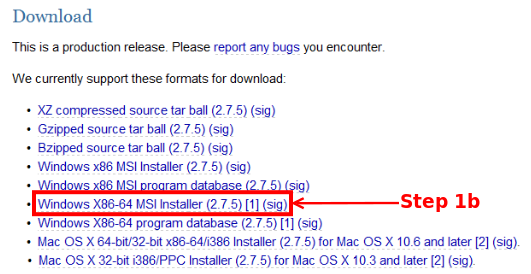
\includegraphics[width=0.6\textwidth]{dia1}
\end{center}
\caption{Link to Python Installer (step 1b.)}
\label{fig:dia1}
\end{figure}
\vfill
{\bf Step 2} (on page 2) will show you how to use this file to Install Python.
\myhrule

% PAGE 2
\newpage
{\Large {\bf Step 2: Installing Python}}
\myhrule
{\bf In this step, you will install Python using the file you downloaded in
Step 1.}
\begin{enumerate}[a.]
\item Locate the file \texttt{python-2.7.5.msi} on your computer. The file
location will depend on your web-browser's download settings.
\item Double-click \texttt{python-2.7.5.msi} to run it.
\item If a `Security Warning' window appears, click ``Run'' (labeled in Figure
\ref{fig:dia2}).
\begin{figure}[h]
\begin{center}
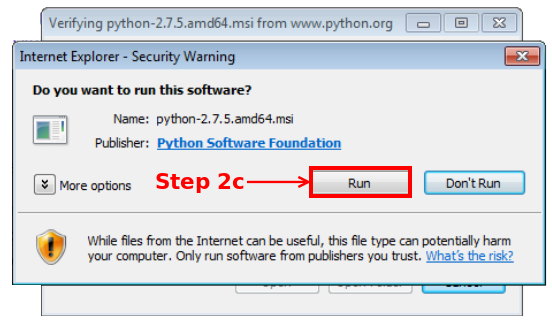
\includegraphics[width=0.4\textwidth]{dia2}
\end{center}
\vspace{-0.5cm}
\caption{``Security Warning'' window (steps 2b. and 3e.)}
\label{fig:dia2}
\end{figure}
\item In the next window, click ``Next'' without changing any settings.
\item Typically, the default installation directory will suffice. To change the
installation directory, select from the drop down menu or type the directory
path in the text box labeled in Figure \ref{fig:dia3}. Click ``Next'' when
done.
\begin{figure}[h]
\begin{center}
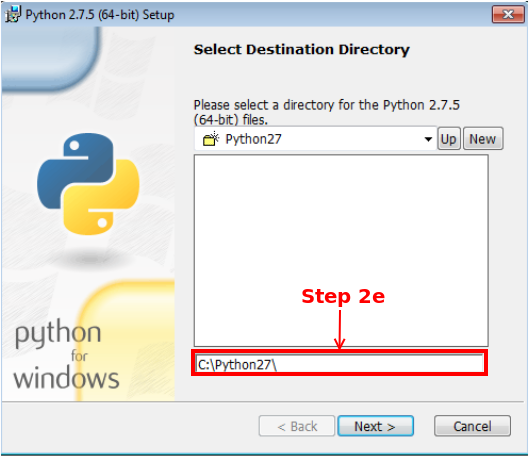
\includegraphics[width=0.45\textwidth]{dia3}
\end{center}
\vspace{-0.5cm}
\caption{Choosing an Installation Directory window (step 2e.)}
\label{fig:dia3}
\end{figure}
\item Click ``Next'' without changing any settings. Wait for the installation
to complete. Then click ``Finish'' to close the installation program.
\end{enumerate}
\vfill
{\bf Step 3} (on page 3) will begin explaining how to configure your computer
to run Python.
\myhrule

% PAGE 3
\newpage
{\Large {\bf Step 3: Opening the Environment Variables Menu}}
\myhrule
{\bf In this step, you will open the Environment Variables Menu in order to
modify Environment Variables. This is necessary for your command line to
run Python files.}
\begin{enumerate}[a.]
\item Open the Start Menu by clicking the bottom left corner of you screen
(labeled in Figure \ref{fig:dia4}).
\item Click on ``Control Panel'' (labeled in Figure \ref{fig:dia4}) to open
the Control Panel.
\begin{figure}[h]
\begin{center}
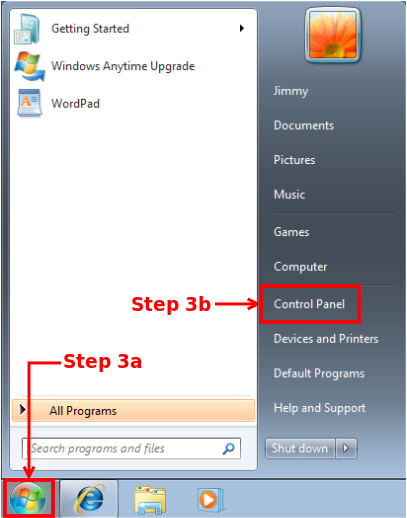
\includegraphics[width=0.35\textwidth]{dia4}
\end{center}
\vspace{-0.5cm}
\caption{The Start Menu (steps 3a. and 3b.)}
\label{fig:dia4}
\end{figure}
\item Type ``advanced'' (without quotes) into the Search Box in the top right
corner of the Control Panel window (as in Figure \ref{fig:dia5}).
\item Click ``View advanced system settings'' (labeled in Figure
\ref{fig:dia5}).
\begin{figure}[h]
\begin{center}
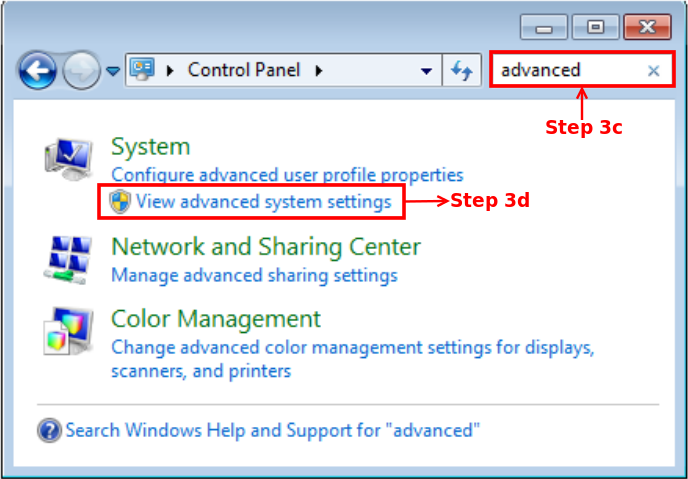
\includegraphics[width=0.6\textwidth]{dia5}
\end{center}
\vspace{-0.5cm}
\caption{The Control Panel (steps 3c. and 3d.)}
\label{fig:dia5}
\end{figure}
\item If a ``User Account Control'' window appears, click ``Yes'' (as in Figure
\ref{fig:dia11}).
\begin{figure}[h]
\begin{center}
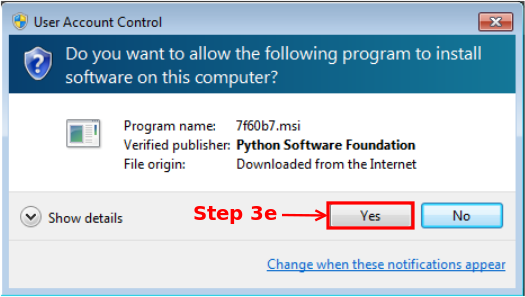
\includegraphics[width=0.6\textwidth]{dia11}
\end{center}
\caption{The User Account Control window (step 3e.)}
\label{fig:dia11}
\end{figure}
\end{enumerate}
\vfill
{\bf Step 4} (on page 5) will show you how to modify the PATH Environment
Variable.
\myhrule

% PAGE 4
\newpage
{\Large {\bf Step 4: Modifying the PATH Environment Variable}}
\myhrule
{\bf In this step, you will modify the PATH environment variable, telling your
command line the location of your Python Installation.}\\

{\bf \color{red} \underline{Warning:}} Important system services depend on
Environment Variables. Do not modify any Environment Variables
except PATH, and do not remove anything from the PATH variable; you should only
{\bf add} information to the PATH variable.

\begin{enumerate}[a.]
\item
\end{enumerate}
\end{document}
